\documentclass[10pt,a4paper]{article}

\usepackage[top=1.2cm, bottom=1.2cm, left=1.2cm, right=1.2cm]{geometry}
\usepackage{paracol}
\usepackage{titlesec}
\usepackage{enumitem}
\usepackage{hyperref}
\usepackage{graphicx}

% Clean links & page setup
\hypersetup{hidelinks}
\pagestyle{empty}
\setlength{\parindent}{0pt}

% Section headers: Clean, ATS-friendly underlined style
\titleformat{\section}{\large\bfseries\uppercase}{}{0em}{}[\titlerule]
\titlespacing*{\section}{0pt}{8pt}{6pt}

\titleformat{\subsection}{\normalsize\bfseries}{}{0em}{}
\titlespacing*{\subsection}{0pt}{6pt}{2pt}

% Tight itemize margins for high readability
\setlist[itemize]{leftmargin=1.2em, topsep=2pt, itemsep=2pt, parsep=0pt}

\begin{document}

% ----------------- HEADER WITH PICTURE -----------------
\begin{minipage}[c]{0.80\textwidth}
    {\Huge \textbf{MOHAMMADHADI KAFI}}\\[4pt]
    {\large \textbf{Senior DevOps \& Infrastructure Engineer}}\\[6pt]
    Email: \href{mailto:mohammadhadikafi@gmail.com}{mohammadhadikafi@gmail.com} \;\textbar\;
    Phone: +98 990 388 8895 \;\textbar\;
    Location: Tehran, Iran\\
    Website: \href{https://hadikafi.me}{hadikafi.me} \;\textbar\;
    LinkedIn: \href{https://www.linkedin.com/in/hadikafi}{linkedin.com/in/hadikafi} \;\textbar\;
    GitHub: \href{https://github.com/hadikafi}{github.com/hadikafi}
\end{minipage}%
\begin{minipage}[c]{0.20\textwidth}
    \raggedleft
    \fbox{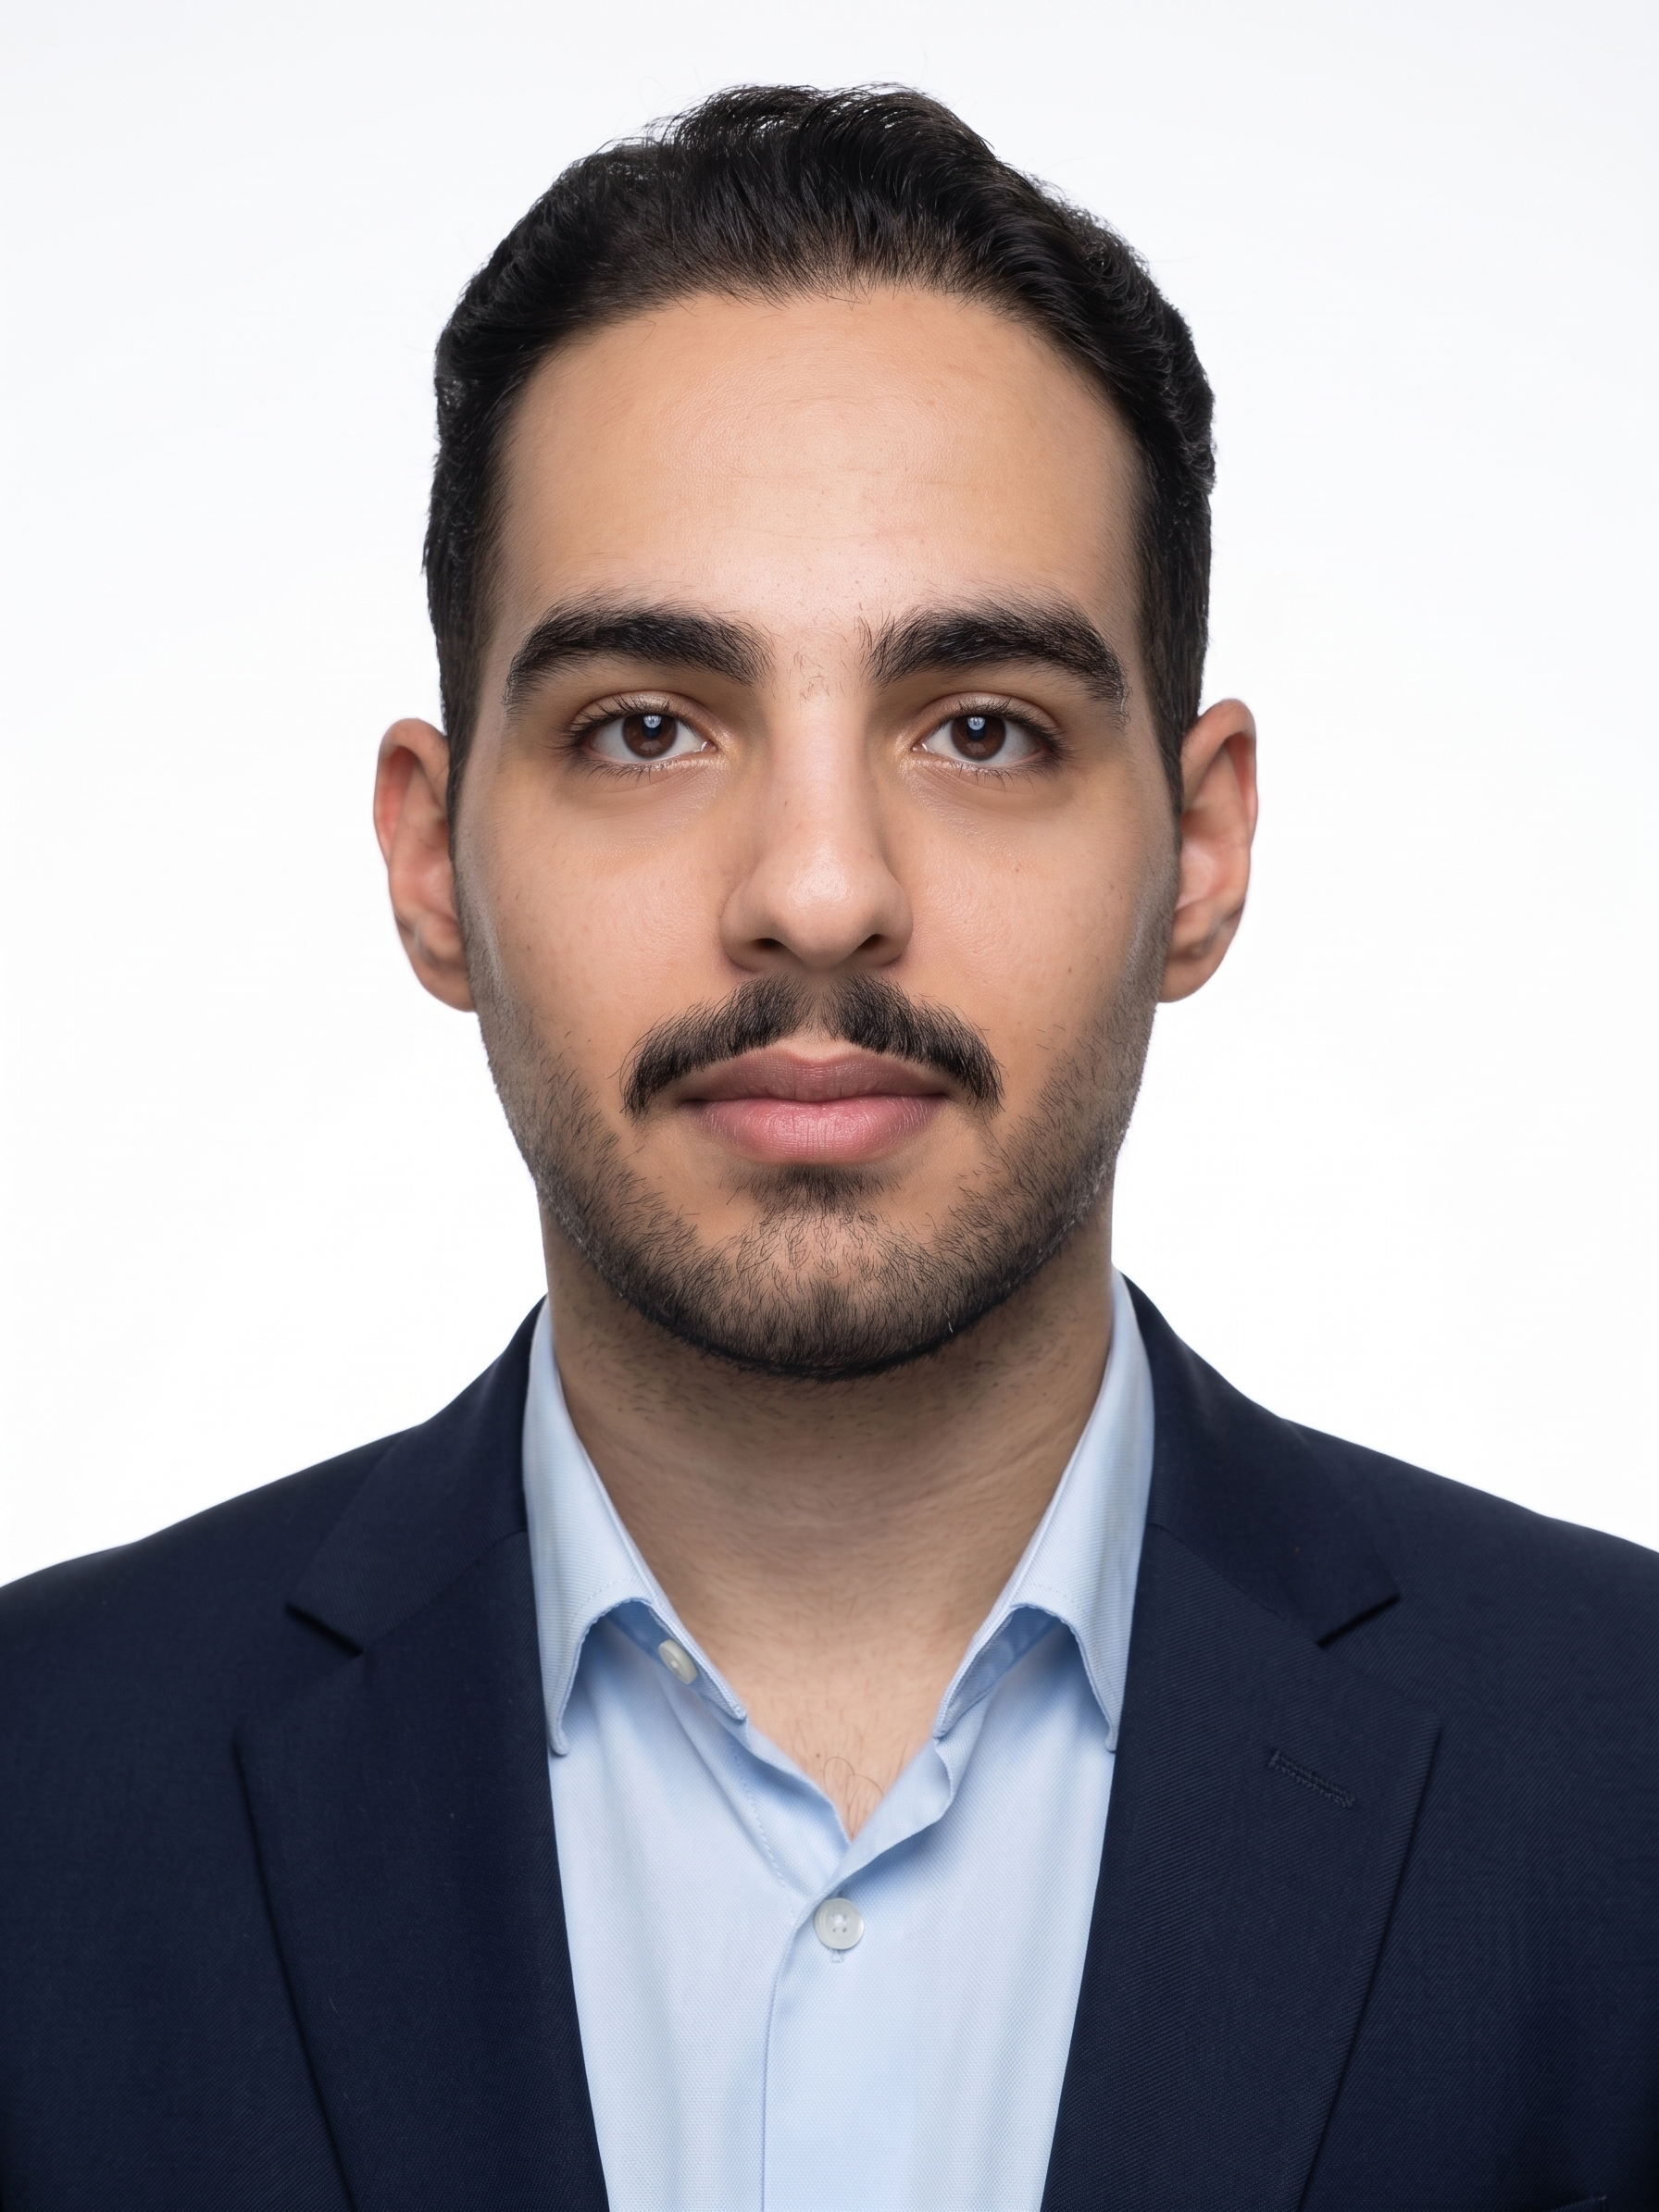
\includegraphics[width=2.5cm,height=3.0cm,keepaspectratio]{profile.jpg}}
\end{minipage}

\vspace{10pt}

% ----------------- 2-COLUMN LAYOUT (68% Main / 32% Sidebar) -----------------
\columnratio{0.68, 0.32}
\setlength{\columnsep}{1.2cm}

\begin{paracol}{2}

% ==================== LEFT COLUMN: SUMMARY, EXPERIENCE, SKILLS & PROJECTS ====================
\section{Summary}
Senior DevOps \& Infrastructure Engineer with extensive experience architecting \textbf{air-gapped} Kubernetes environments, \textbf{bare-metal} AI compute clusters, and resilient data streaming pipelines. Proven track record in supporting mission-critical banking platforms with \textbf{zero-downtime} requirements, building fault-tolerant database architectures, and maintaining service reliability and disaster recovery through upstream connectivity outages.

\vspace{4pt}

\section{Work Experience}

\textbf{AdanAI} \hfill \textit{Tehran, Iran}\\
\textbf{DevOps Engineer} \hfill \textit{Mar 2026 -- Present}
\begin{itemize}
    \item Maintain \textbf{zero-downtime} operations for ``\textbf{Dima},'' a mission-critical AI banking assistant (\textbf{Bank Mellat}), by redesigning and optimizing load balancing and failover architectures.
    \item Provisioned and configured \textbf{bare-metal} AI infrastructure from scratch, setting up a Dell PowerEdge XE9680 server equipped with $8\times$ \textbf{NVIDIA H200} GPUs.
    \item Deployed and optimized the Qwen 3.6 model for production inference using vLLM, tuning serving parameters to achieve maximum throughput and low latency.
    \item Architected high-availability (HA) infrastructure for ``\textbf{Narenjestan},'' a RAG-powered internal AI assistant supporting \textbf{Bank Mellat} branch personnel with on-demand technical queries; deployed fault-tolerant clusters for Elasticsearch, Qdrant, PostgreSQL, MongoDB, and Redis.
    \item Deployed internal Sonatype Nexus instances to cache build dependencies and maintain uninterrupted \textbf{CI/CD} workflows during broad network and upstream internet outages.
    \item Built self-hosted collaboration infrastructure (Nextcloud with integrated chat and video conferencing), ensuring secure remote work and internal communication through connectivity blackouts.
    \item Engineered \textbf{automated}, offsite virtual machine backup and disaster recovery pipelines to safeguard critical systems and state against physical datacenter threats.
\end{itemize}

\vspace{8pt}

\textbf{Pooya} \hfill \textit{Tehran, Iran}\\
\textbf{DevOps Engineer} \hfill \textit{Sep 2022 -- Mar 2026}
\begin{itemize}
    \item Built and maintained an on-premise Kubernetes cluster (3 Control Plane, 9 Worker nodes) in a restricted, \textbf{air-gapped} network for enterprise workloads.
    \item Provisioned high-throughput data and streaming clusters inside Kubernetes---including Kafka, ClickHouse, Apache Spark, MongoDB, MinIO, and Redis---powering an online fraud detection platform for \textbf{Bank Refah}.
    \item Migrated internal teams from manual deployments to \textbf{automated} \textbf{CI/CD} pipelines using Jenkins and Argo CD, standardizing delivery workflows.
    \item Deployed and configured Sonatype Nexus as a centralized artifact and proxy repository to resolve \textbf{air-gapped} dependency management across build systems.
    \item \textbf{Automated} OS-level configuration, recurring maintenance, and security patch rollouts across Linux servers using Ansible playbooks.
    \item Implemented deep database observability by integrating dedicated Prometheus exporters (MongoDB and Oracle exporters) into production clusters.
    \item Designed unified Grafana dashboards covering host metrics, service \textbf{SLAs}, and business-level transactions for maintained systems.
    \item Deployed centralized logging stacks with Grafana Loki and containerized legacy backend services with Docker.
\end{itemize}

\vspace{8pt}

\section{Technical Skills}

\textbf{AI Infra \& LLM Serving:} vLLM, \textbf{NVIDIA H200} GPUs, CUDA, Dell PowerEdge XE9680, Qwen Models, Model Inference Optimization\\[3pt]
\textbf{Orchestration \& Containers:} Kubernetes (\textbf{Air-Gapped}, \textbf{Bare-Metal}), Docker, Docker Compose, Argo CD (GitOps), Jenkins, Ansible\\[3pt]
\textbf{Observability \& Monitoring:} Prometheus, Alertmanager, Grafana Dashboards, Loki, ELK Stack, Distributed Tracing, DB Exporters\\[3pt]
\textbf{Databases \& Streaming:} ClickHouse, Kafka, Apache Spark, PostgreSQL HA, Oracle, MongoDB Clusters, Redis HA/Sentinel, Qdrant, MinIO\\[3pt]
\textbf{Networking \& Systems:} Linux (Ubuntu, Rocky Linux), TCP/IP, UDP, DNS, DHCP, TLS/SSL, WebSockets (WS), Nginx Reverse Proxies, MikroTik (RouterOS, Mangle, Wireless), Cisco Catalyst Switching, Sonatype Nexus, Harbor, High Availability / DR

\vspace{8pt}

\section{Key Projects}

\textbf{Corporate Multi-Site Network Infrastructure} \hfill \textit{Enterprise Project}
\begin{itemize}
    \item Designed and executed complete active and passive network infrastructure from ground up for an enterprise office accommodating 20+ staff members, integrating Cisco Catalyst switches and MikroTik edge routers.
    \item Established an inter-office Point-to-Point (PtP) wireless bridge using MikroTik LHG 5 ax radios; analyzed spectral interference and optimized channel frequencies to deliver stable, high-throughput transmission.
    \item Implemented policy-based routing (PBR) on MikroTik RouterOS using firewall Mangle rules and dynamic address lists, achieving domestic vs. international traffic separation.
\end{itemize}

\switchcolumn

% ==================== RIGHT COLUMN: EDUCATION, DETAILS, LANGUAGES & CORE FOCUS ====================
\section{Education}

\textbf{M.Sc. in Computer Engineering -- Software} \\
\textit{Khatam University} \\
2024 -- Present

\vspace{8pt}

\textbf{B.Sc. in Computer Engineering} \\
\textit{Babol Noshirvani University of Technology} \\
Graduated: 2024

\vspace{12pt}

\section{Personal Details}

\textbf{Location / Residence:} \\
Central Tehran, Iran

\vspace{6pt}

\textbf{Date of Birth:} \\
2000/09/30

\vspace{6pt}

\textbf{Military Service:} \\
Educational Exemption

\vspace{12pt}

\section{Languages}

\textbf{Persian:} Native \\
\textbf{English:} Professional Working Proficiency

\vspace{12pt}

\section{Core Focus}

\begin{itemize}
    \item High-Availability Systems
    \item \textbf{Air-Gapped} Environments
    \item \textbf{Bare-Metal} AI Deployments
    \item Disaster Recovery / Backups
    \item Multi-Site Enterprise Networks
    \item Telecom \& Banking Platforms
\end{itemize}

\end{paracol}

\end{document}